\documentclass[12pt,a4paper]{article}

\usepackage[utf8]{inputenc}
\usepackage[T2A]{fontenc}
\usepackage[ukrainian]{babel}
\usepackage[a4paper, margin=2cm]{geometry}

\usepackage{amsmath, amssymb, amsthm}
\usepackage[most]{tcolorbox}
\usepackage{graphicx}
\usepackage{caption}
\usepackage{fancyhdr}

\pagestyle{fancy}
\fancyhf{}
\rhead{Лабораторна робота № 9--10}
\lhead{Завдання 2}
\cfoot{\thepage}

\setlength{\parindent}{1.25cm}
\setlength{\parskip}{0.2cm}

\newtheorem{theorem}{Теорема}

\begin{document}

\begin{center}
    {\LARGE \textbf{Трикутник та його властивості}}
\end{center}

\section*{Теоретичні відомості}

\begin{tcolorbox}[colback=blue!10!white, colframe=blue!60!black, title=Означення]
Трикутник --- це геометрична фігура, яка складається з трьох точок, що не лежать на одній прямій, і трьох відрізків, які попарно сполучають ці точки.
\end{tcolorbox}

Трикутник є однією з основних фігур планіметрії. Він має три сторони, три кути та три вершини. Сума внутрішніх кутів будь-якого трикутника дорівнює $180^\circ$.

Основні позначення:
\[
\triangle ABC
\]
де $A$, $B$, $C$ --- вершини трикутника, а $AB$, $BC$, $CA$ --- його сторони.

\subsection*{Основні властивості трикутника}

\begin{enumerate}
    \item Сума внутрішніх кутів трикутника дорівнює $180^\circ$.
    \item Будь-яка сторона трикутника менша від суми двох інших сторін.
    \item Більша сторона лежить проти більшого кута.
    \item Якщо дві сторони трикутника рівні, то він рівнобедрений.
\end{enumerate}

\begin{theorem}
Сума внутрішніх кутів трикутника дорівнює $180^\circ$.
\label{th:sum_angles}
\end{theorem}

\begin{proof}
Нехай дано трикутник $\triangle ABC$. Проведемо через вершину $A$ пряму, паралельну стороні $BC$. Тоді кути, утворені цією прямою зі сторонами $AB$ і $AC$, будуть відповідно рівні кутам при вершинах $B$ і $C$ як внутрішні різносторонні.

Отже, на розгорнутому куті при точці $A$ маємо суму трьох кутів:
\[
\angle A + \angle B + \angle C = 180^\circ.
\]

Теорему доведено.
\end{proof}

\section*{Формули}

Для трикутника використовуються такі формули:

\begin{equation}
P = a + b + c
\end{equation}
де $P$ --- периметр трикутника.

\begin{equation}
S = \frac{1}{2}ah
\end{equation}
де $a$ --- сторона трикутника, $h$ --- висота, проведена до цієї сторони.

Для прямокутного трикутника виконується теорема Піфагора:
\begin{equation}
c^2 = a^2 + b^2
\end{equation}
де $c$ --- гіпотенуза, а $a$ і $b$ --- катети.

\section*{Приклад пояснення}

Розглянемо трикутник зі сторонами $3$ см, $4$ см і $5$ см. Оскільки
\[
5^2 = 3^2 + 4^2,
\]
тобто
\[
25 = 9 + 16,
\]
то даний трикутник є прямокутним.

Обчислимо його периметр:
\[
P = 3 + 4 + 5 = 12 \text{ см}.
\]

Обчислимо площу:
\[
S = \frac{1}{2} \cdot 3 \cdot 4 = 6 \text{ см}^2.
\]

Як показано в теоремі \ref{th:sum_angles}, сума кутів цього трикутника також дорівнює $180^\circ$.

\section*{Ілюстрація}

На рисунку \ref{fig:triangle} зображено трикутник $ABC$.

\begin{figure}[h!]
    \centering
    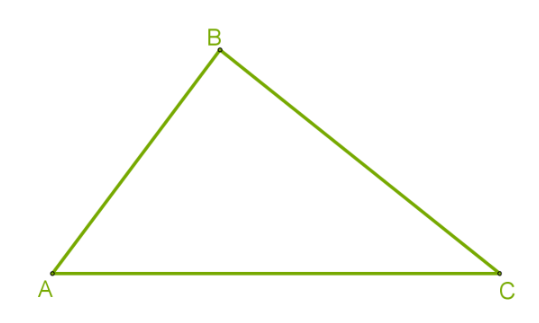
\includegraphics[width=0.45\textwidth]{triangle.png}
    \caption{Зображення трикутника $ABC$}
    \label{fig:triangle}
\end{figure}

\section*{Висновок}

У цій роботі було створено документ у LaTeX на тему «Трикутник та його властивості». У документі використано кольоровий блок означення, теорему, доведення, математичні формули, нумерований список та рисунок із підписом і посиланням у тексті. Це дозволяє зручно оформлювати математичні тексти та автоматизувати їх структурування.

\end{document}